\documentclass{amsart}
\usepackage{amsfonts, amsthm, amssymb, amsmath}
\usepackage{mathtools}
\usepackage{graphicx,caption,subcaption}
\usepackage{comment}
\usepackage{xcolor}
\usepackage{tikz}
%\usetikzlibrary{decorations.markings,arrows.meta,calc,fit,quotes,cd,math,external}
\usetikzlibrary{
  matrix,
  arrows,
  arrows.meta,
  calc,
  fit,
  quotes,
  cd,
  math,
  external,
  shapes,
  decorations.markings,
  decorations.pathreplacing,
  patterns,
  decorations.pathmorphing
}

\usepackage{url}
\usepackage[inline]{enumitem}
	\setlist{itemsep=0em, topsep=0em, parsep=0em}
	\setlist[enumerate]{label=(\alph*)}
\usepackage[all,2cell]{xy}\UseAllTwocells\SilentMatrices
\usepackage[breaklinks=true]{hyperref}%John's choices, can change; previous choice \definecolor{hyperrefcolor}{rgb}{0,0,0.7}
\definecolor{darkgreen}{rgb}{0,0.45,0}
\definecolor{myurlcolor}{rgb}{0.6,0,0}
\definecolor{mycitecolor}{rgb}{0,0,0.8}
\definecolor{myrefcolor}{rgb}{0,0,0.8}
\hypersetup{colorlinks, linkcolor=myrefcolor, citecolor=darkgreen, urlcolor=myurlcolor,
final,linktoc=page}
\usepackage[capitalize]{cleveref}
\crefname{equation}{}{}
\crefname{item}{}{}
\crefname{prop}{Proposition}{Propositions}

%
% environments and counters
%

\newtheorem{thm}{Theorem}[section]
\newtheorem{cnj}[thm]{Conjecture}
\newtheorem{lem}[thm]{Lemma}
\newtheorem{prop}[thm]{Proposition}
\newtheorem{cor}[thm]{Corollary}

\theoremstyle{remark}
	\newtheorem{remark}[thm]{Remark}
	\newtheorem{notation}[thm]{Notation}

\theoremstyle{definition}
	\newtheorem{ex}[thm]{Example} 
	\newtheorem{defn}[thm]{Definition}

% math text formatting
\newcommand{\cat}[1]{\mathsf{#1}}

% common category names

\newcommand{\Set}{\cat{Set}}
\newcommand{\Grph}{\cat{Grph}}
\newcommand{\Cat}{\cat{Cat}}
\newcommand{\twoCat}{\cat{2Cat}}
\newcommand{\Adj}{\cat{Adj}}
\newcommand{\one}{\mathbf{1}}
\newcommand{\two}{\mathbf{2}}
\newcommand{\Fib}{\cat{Fib}}
\newcommand{\OpFib}{\cat{OpFib}}
\newcommand{\Corefl}{\cat{Corefl}}
\newcommand{\Rali}{\cat{Rali}}

\newcommand{\C}{\cat{A}}
\newcommand{\D}{\cat{X}}
\newcommand{\A}{\cat{A}}
\newcommand{\X}{\cat{X}}
\newcommand{\U}{U}
\newcommand{\Q}{Q}
\renewcommand{\L}{L}
\newcommand{\R}{R}
\renewcommand{\P}{P}
\newcommand{\B}{\cat{B}}
\newcommand{\Y}{\cat{Y}}

\newcommand{\Cocart}{\mathrm{Cocart}}
\newcommand{\Cart}{\mathrm{Cart}}

\newcommand{\op}[1]{\operatorname{#1}}
\renewcommand{\t}[1]{\text{#1}}

\newcommand{\from}{\colon}
\newcommand{\xto}[1]{\xrightarrow{#1}}
\newcommand{\To}{\Rightarrow}
\newcommand{\Tto}{\Rrightarrow}
\newcommand{\bydef}{\coloneqq}
\newcommand{\define}{\textbf}%consider change to bold? or something else?

%
% math operators
%

\DeclareMathOperator{\Hom}{Hom}
\DeclareMathOperator{\id}{id}
\DeclareMathOperator{\ob}{Ob}
\DeclareMathOperator{\arr}{arr}
\DeclareMathOperator{\im}{im}
\DeclareMathOperator{\Aut}{Aut}
\DeclareMathOperator{\Bij}{Bij}
\DeclareMathOperator{\Sub}{Sub}
\DeclareMathOperator{\colim}{colim}
\newcommand{\iso}{\cong}

%
% tikz styles
%

% arrows for commuting diagram
\tikzset{
  cd/.style={
    ->,
    scale=6,
    >=angle 90,
    font=\scriptsize}
  }

% its us!

\definecolor{purple(x11)}{rgb}{0.5, 0.0, 0.5}
\newcommand{\chris}{\color{purple(x11)}}
\newcommand{\daniel}{\color{red}}


\begin{document}
\title{A note on Fibrations and Adjunctions}

\author{Daniel Cicala and Christina Vasilakopoulou} 
\address{Departement of Mathematics, University of California, Riverside, 900 University Avenue, 92521, USA}
\email{cicala@math.ucr.edu,vasilak@ucr.edu}

\begin{abstract}
Fibrations and Adjunctions rock.
\end{abstract}

\maketitle

\tableofcontents


\section{Introduction}

-Discuss how for the existence of a left adjoint we would expect some limit preserving condition. This story is a different way of sailing.
-Strictness conditions and evilness conditions. Getting rid of them later due to Street notion.

\section*{Things To Do}
\begin{itemize}
\item 
\end{itemize}

\section*{Acknowledgements} We would like to thank John Baez, Claudio Hermida, Steve Lack, ... for invaluable advice and discussions.

\section{Preliminaries}\label{sec:preliminaries}

\subsection*{Grothendieck Opfibrations}
We recall some basic material from the theory of fibrations; standard references include  \cite{Grayfibredandcofibred,hermidaphd,Handbook2}. 
For our purposes, we center our presentation mostly around opfibrations.

Consider a functor $\U \colon\X \to \A$. A morphism $\beta \colon x \to y$ in $\X $ over a morphism $f = \U(\beta) \colon a \to b$ in $\A$ is called \define{cocartesian} if and only if, for all $g \colon b \to b'$ in $\A$ and $\gamma \colon x\to y'$ in $\X $ with $\U(\gamma) = g\circ f$, there exists a unique $\delta \colon y\to y'$ in $\X$ such that $\U(\delta) = g$ and $\gamma = \delta \circ \beta$:
\begin{equation}\label{eq:opfibration}
\xymatrix @R=.1in @C=.6in
{&& y'\ar @{.>}@/_/[dd] &&\\
x\ar[r]_-{\beta} \ar @{.>}@/_/[dd]
\ar[urr]^-{\gamma} & 
y \ar @{.>}@/_/[dd] \ar @{-->}[ur]_-{\exists! \delta}
&& \textrm{in }\X\\
&& b' &&\\
a\ar[r]_-{f=\U\beta} \ar[urr]^-{g\circ f=\U\gamma}
 & b \ar[ur]_-g && \textrm{in }\A}
\end{equation}
For any object $a\in\A$, we denote by $\X_a$ the \define{fibre} of $U$ over $a$, i.e. the subcategory of $\X$ which consists of objects $x$ above $a$, namely $\U(x) = a$, and vertical morphisms $\beta$, namely $\U(\beta) = 1_a$. The functor $\U \colon \X \to \A$ is an \define{opfibration} if and only if, for all $f \colon a \to b$ in $\A$ and $x\in\X_a$, there is a cocartesian morphism $\beta$ with domain $x$ above $f$; it is called a \define{cocartesian lifting} of $b$ along $f$. The category $\A$ is called the \define{base} of the opfibration, and $\X $ its \define{total category}.
Of course, this is a dual notion to that of a \define{fibration}.

For any opfibration $\U\colon \X \to\A$, assuming the axiom of choice we may select a cocartesian arrow over each $f\colon a\to b$ in $\A$ and $x\in\X_a$, denoted by $\Cocart(f,x)\colon x\to f_!(x)$. Such a choice of cocartesian liftings is called a \define{cleavage} for $\U$, which is then called a \define{cloven opfibration}; in this way, any opfibration can be assumed to be cloven. As a special case of the universal property, any arrow in the total category of an opfibration factorizes uniquely into a cocartesian morphism followed by a vertical one:
\begin{equation}\label{factor}
\xymatrix @C=.6in @R=.3in
{x \ar @{.>}[dd]\ar[rr]^\gamma \ar[drr]_-{\Cocart(f,x)} && y &\\
&& f_!x \ar @{-->}[u]_-{\delta} \ar @{.>}[d] & \textrm{in }\X  \\
a\ar[rr]_-{f} && b & \textrm{in }\A.}
\end{equation}
The choice of cocartesian liftings in a cloven opfibration induces a so-called \define{reindexing functor} between the fibre categories
\begin{equation}\label{reindexing}
 f_!\colon\X_a\to\X_b
\end{equation}
for any $f\colon a\to b$ in the base category. It can be verified by the cocartesian lifting property that $(1_a)_!\cong1_{\X_a}$ and $(f\circ g)_!\cong f_!\circ g_!$. If these isomorphisms are equalities, we have the notion of a \define{split} (op)fibration.

For what follows, it is necessary to clarify the relation between the existence of colimits in the total category of an opfibration to the existence of those colimits in the fibres in a coherent way. For more details, and a proof of the following result, see \cite[Cor. 3.7]{FibredAdjunctions}.

\begin{lem}\label{lem:fibrewiselimits}
Suppose $\cat{J}$ is a small category and $\U\colon\X\to\A$ is an opfibration. If the base $\A$ has $\cat{J}$-colimits,
the following are equivalent:
\begin{enumerate}
 \item all fibres have $\cat{J}$-colimits, and the reindexing functors preserve them; \label{it:2}
 \item the total category $\X$ has $\cat{J}$-colimits, and $\U$ (strictly) preserves them.
\end{enumerate}
\end{lem}
The above formulation and its dual version relate opfibrations specifically with colimits and fibrations with limits. Notice that condition \ref{it:2} is the usual formal definition of when an arbitrary opfibration has \emph{opfibred $\cat{J}$-colimits}, which in principle does not require a $\cat{J}$-
cocomplete base. The strict preservation of colimits is discussed in detail below \cref{lem:isofactid}.

{\chris Categories of opfibrations, depending on section 4}

\subsection*{Street Opfibrations}

While fibrations are well-studied and frequently used
without hesitation, there is an ``evilness'' about them. The
term ``evil'' is a tongue-in-cheek expression applied to any
categorical concept that fails to transport across an
equivalence of categories.  The aspect of a fibration
$ \U \from \X \to \A $ that fails occurs when, given any arrow
$ f \from a \to b $ and cartesian lift
$ \theta \from x \to y $ where $ y $ is in the fiber of
$ b $, we require that $ Ux $ \emph{equals} $ a $.  After
rebasing $ U $ with an equivalent category, it is entirely
possible that the equality weakens to an isomorphism meaning
that the rebased version of $ U $ is no longer a
fibration. In general, evil practices in category theory are
morally dubious. Fibrations, however, frequently get a pass
because for concrete categories, fibrations do satisfy this
strict equality.  However, there is a non-evil version of a
fibration.

\begin{defn}[Street fibration]

  A functor $ U \from \X \to \A $ is a \define{Street
    fibration} if, for any arrow $ f \from a \to b $ in $ \A
  $ and $ y $ in the fiber of $ b $, there exists a
  cartesian lifing $ \theta \from x \to y $ and an
  isomorphism $ h \from Ux \iso a $ such that $ fh = U\theta $
  
\end{defn}

In the Street fibration, the evil equality is replaced by an
isomorphism $ h $.  One can readily check that rebasing a
\emph{Street fibration} $ U $ with an equivalent category
does, in fact, give another Street fibration.

Because we generalize our results in Section
\ref{sec:groth-fibs-ralis} from Grothendieck fibrations to
Street fibrations, we need a generalized version of Lemma
\ref{lem:fibrewiselimits}.

\begin{lem} \label{lem:street-fibrewise-limits}
  Suppose $ \cat{J} $ is a small category and $ U \from \X
  \to \A $ is a Street (op)fibration. If $ \A $ has $ \cat{J}
  $-(co)limits, the following are equivalent:
  \begin{enumerate}
  \item
    all fibres have $ \cat{J} $-colimits and the
    reindexing functors preserve them;
  \item
    $ \X $ has $ \cat{J} $-(co)limits and $ U $ preserves
    them.
  \end{enumerate}
\end{lem}

\begin{proof}
  Every Street fibration can be factored as a Grothendieck
  fibration followed by an equivalence of categories.  This
  lemma holds for Grothendieck fibrations plus categories having
  (co)limits and functors preserving them are both properties
  that satisfy the principle of equivalence.  
\end{proof}

\subsection*{Choice of colimits}

In what follows, and in particular for our main \cref{thm:mainthm}, we often require that certain colimits must be \emph{strictly} preserved. Whereas such an uncommon condition sounds `evil' at first, we remark that it is the necessary such in order to match to the inherent `evilness' of Grothendieck fibrations. Moreover, in \cref{Streetfibs} we examine the non-strict context which then naturally matches to the notion of a Street fibration as discussed above.

In more detail, assuming the axiom of choice we can regard any category with (co)limits as having \emph{chosen} ones, in the sense of choosing a specific adjoint (out of all isomorphic ones) to the constant diagram functor:
\begin{displaymath}
 \begin{tikzcd}[sep=.7in]
 \cat{C}\ar[r,pos=.6,"\Delta_\cat{C}"description]\ar[r,phantom,bend left=18,pos=.6,"\bot"]\ar[r,phantom,bend right=18,pos=.6,"\bot"] &  {[}\cat{J},\cat{C}{]}\ar[l,bend right,pos=.4,"\colim_\cat{J}"']\ar[l,bend left,pos=.4,"\lim_\cat{J}"]
 \end{tikzcd}
\end{displaymath}
Some categories, like $\Set$, even have a canonical choice corresponding to well-known constructions of (co)limits of sets. In general, a functor $F\colon\cat{C}\to\cat{D}$ between categories with colimits, for example, preserves them when the following diagram
\begin{equation}\label{eq:preservelimits}
  \begin{tikzcd}
\phantom{A}[\cat{J},\cat{C}]\ar[r,"\colim"]\ar[d,"{[\cat{J},F]}"']\ar[dr,phantom,"\cong"] & \cat{C}\ar[d,"F"] \\
\phantom{A}[\cat{J},\cat{D}]\ar[r,"\colim"'] & \cat{D}
  \end{tikzcd}
 \end{equation}
which is the \emph{mate} of the commutative square with $\Delta$'s, commutes up to natural isomorphism.
The following two lemmas (due to Steve Lack) present two natural settings where functors between categories with chosen (co)limits \emph{strictly} preserve them; evidently, such a thing is to be expected only when the limits in the categories have been both previously constructed from chosen limits in some fixed category.
\begin{lem}\label{lem:Lack1}
 Suppose $\cat{C}$ is a category with chosen (co)limits (of any class). Then for any two categories $\cat{A}$ and $\cat{B}$ and any functor $F\colon\cat{A}\to\cat{B}$ between them, the pre-composition functor
 \begin{displaymath}
  \begin{tikzcd}[row sep=.05in]
  F^*\colon[\cat{B},\cat{C}]\ar[r] & \;[\cat{A},\cat{C}] \\
  \;\;\;\;\cat{B}\xrightarrow{H}\cat{C}\ar[r,mapsto] & \cat{A}\xrightarrow{F}\cat{B}\xrightarrow{H}\cat{C}
  \end{tikzcd}
 \end{displaymath}
strictly preserves the chosen (co)limits.
\end{lem}
\begin{proof}
 This follows from the pointwise construction of colimits in functor categories.
\end{proof}

As a particular case, the following result concerns our motivating example.
\begin{cor}
There is a canonical choice of (co)limits in $\Grph$ inherited from those in $\Set$ so that the domain and codomain functors $\Grph\to\Set$ strictly preserve all limits and colimits.
\end{cor}

\begin{proof}
 Consider the two functors $1,2\colon\one{=}\{\bullet\}\longrightarrow\{1\rightrightarrows2\}{=}\two$. Choosing the canonical (co)limits in $\Set$, by \cref{lem:Lack1} we obtain two functors
\begin{displaymath}
\begin{tikzcd}
 \Grph=[\two,\Set]\ar[r,shift left,"\mathrm{dom}"]\ar[r,shift right,"\mathrm{cod}"'] & \;[\one,\Set]=\Set
 \end{tikzcd}
\end{displaymath}
that strictly preserve them.
\end{proof}

The following case again follows from a construction of chosen limits in common ground; colimits adhere to a dual result.
\begin{lem}
Suppose $\cat{C}$ and $\cat{D}$ have chosen limits and $F\colon\cat{C}\to\cat{D}$ is an arbitrary functor. Then the comma category $F\downarrow\cat{D}$ can be equipped with limits in such a way that both projections $\cat{C}\leftarrow F\downarrow\cat{D}\to\cat{D}$ strictly preserve them.
\end{lem}

\begin{proof}
 This follows from the canonical construction of limits in comma categories, as found e.g.\ in~\cite[\S 2.16]{Handbook1}.
\end{proof}

Finally, another class of functors which is notable when it comes to strict preservation of (co)limits are (op)fibrations. In more detail, there is no loss of generality for a colimit-preserving opfibration if we assume that colimits are in fact preserved on-the-nose, whereas such a statement does definitely not apply to arbitrary functors. This is due to the following lemma, which is a special case of a more general fact: the embedding of $\OpFib$ in the 2-category $\OpFib_{\sim}$ where 2-cells are squares filled with isomorphisms, is locally fully faithful and essentially surjective (also for fibs...references...\cite{Fib2Fib}?). We thank Claudio Hermida for these observations.
\begin{lem}\label{lem:isofactid}
 Suppose $\U$ and $\Q$ are opfibrations, and there is a natural isomorphism
 \begin{displaymath}
  \begin{tikzcd}
\X\ar[r,"H"]\ar[d,"\U"']\ar[dr,phantom,"\stackrel{\phi}{\cong}"] & \Y\ar[d,"\Q"] \\
\A\ar[r,"F"'] & \B
  \end{tikzcd}
 \end{displaymath}
Then $\phi$ factors as a commutative square composed by an isomorphism $\hat{\phi}$, as in
 \begin{displaymath}
  \begin{tikzcd}[row sep=.15in]
\X\ar[rr,bend left,"H"]\ar[rr,bend right,"\widehat{H}"']\ar[rr,phantom,"{\stackrel{\hat{\phi}}{\cong}}"description]\ar[dd,"\U"'] && \Y\ar[dd,"\Q"] \\
\hole \\
\A\ar[rr,"F"'] && \B
  \end{tikzcd}
 \end{displaymath}
\end{lem}
As a result, if $\U$ is an opfibration that preserves $\cat{J}$-colimits for some small $\cat{J}$, we can factor the natural isomorphism \cref{eq:preservelimits}, where the left leg is also a fibration, as
\begin{displaymath}
  \begin{tikzcd}[row sep=.15in]
{[\cat{J},\cat{X}]}\ar[rr,bend left,pos=.4,"\colim"]\ar[rr,bend right,pos=.4,"\widehat{\colim}"']\ar[rr,phantom,"\cong"description]\ar[dd,"{[\cat{J},\U]}"'] && \X\ar[dd,"\U"] \\
\hole \\
{[\cat{J},\cat{A}]}\ar[rr,"\colim"'] && \A
  \end{tikzcd}
 \end{displaymath}
essentially changing the choice of colimits in the total category and establishing that $Q$ now strictly preserves them. In a dual way, we may assume that any fibration strictly preserves chosen limits, if it preserves limits in the ordinary sense.

\subsection*{Sketch notes for Claudio}

I am trying to reason in a similar way to the above (possibly) to be able to say that the first clause of \cref{lem:fibrewiselimits} could be expressed as `chosen colimits such that the reindexing functors STRICTLY preserve them'. Or understand why it is not possible to say that.

Denote by $PB$ the pullback of bottom $\Delta$ and $[\cat{J},\U]$. 
\begin{displaymath}
 \begin{tikzcd}
  \X\ar[drr,bend left,"\Delta"]\ar[ddr,bend right,"\U"']\ar[dr,dotted,"F"] && \\
  &PB\ar[r]\ar[d] & {[\cat{J},\cat{X}]}\ar[d,"{[\cat{J},\U]}"] \\
  &\A\ar[r, bend right, pos=.6, "\Delta"']\ar[r,phantom,"\bot"description] & {[\cat{J},\A]}\ar[l,bend right,pos=.4,"\colim"']
 \end{tikzcd}
\end{displaymath}
The following are equivalent:
\begin{enumerate}
 \item there exists a left adjoint $\colim$ to the top $\Delta$ such that the outside square forms an adjunction in $\OpFib$
 \item there exists a left adjoint $G$ to the middle $F$ such that the triangle forms an adjunction in $\OpFib(\A)$
\end{enumerate}
%Above we established that any opfibration may be assumed to strictly preserve colimits, by changing the chosen colimit functor in the total category.
The adjunction $G\dashv F$ consists of fibrewise adjunctions $G_a\dashv F_a$ which by construction of the pullback, where it can be seen that $PB_a\cong[\cat{J},\X_a]$, precisely give the existence of colimits in the fibres (namely each $G_a$ is a colimit functor $[\cat{J},\X_a]\to\X_a$). So far so good. 

By the fact that left adjoints in $\cat{Cat}^2$ or the slices automatically preserve cocartesian liftings, we get that $f_!(\colim_a H)\cong \colim_b (f_!H)$ for any $f\colon a\to b$ in $\A$, namely a natural isomorphism square
\begin{displaymath}
 \begin{tikzcd}
 \phantom{A}[\cat{J},\cat{X}_a]\ar[r,"\colim_a"]\ar[d,"f_!\circ-"']\ar[dr,phantom,"\cong"] & \cat{X}_a\ar[d,"f_!"] \\
\phantom{A}[\cat{J},\cat{X}_b]\ar[r,"\colim_b"'] & \cat{X}_b 
 \end{tikzcd}
\end{displaymath}

So it is clear that the reindexing functors preserve colimits in the usual sense, up to isomorphism. However, this time I do not see how to use \cref{lem:isofactid} like I did before to show that $\U$ strictly preserves colimits. This isomorphism square is NOT a square of two opfibrations and two functors, like before!

As a result, I do not see how the previous `strictification' result can help now.


\subsection*{Coreflections and laris}

We will use the acronym \emph{lari}, originally introduced in~\cite{Grayfibredandcofibred}, for the notion of a `left adjoint, right inverse' functor. Explicitly, if $\U\colon\cat{D}\to\cat{C}$ has a lari $\L$, then $\L\dashv \U$ and $\eta\colon1_\cat{C}=\U\L$. Equivalently, in this case we can say that $\U$ is a \emph{rali}, namely it is a right adjoint, left inverse of some $\L$ --- still the unit of the adjunction is the identity, with $\U$ now being a left inverse. Analogously, if a functor has a \emph{rari} or equivalently is a \emph{lali}, then the counit of the adjunction is the identity.

Both these notions are special cases of the well-known notions of \emph{(co)reflections}, i.e. ...
{\chris Position here the well-known equivalences clauses for coreflections, also their strict versions for laris.}
\begin{prop}\label{prop:coreflection}
 The following are equivalent for an adjunction $\L\dashv\U\colon\D\to\C$:
 \begin{enumerate}
  \item $\L$ is strictly fully faithful (resp. fully faithful);
  \item the unit $\eta\colon1_\C\Rightarrow \U\L$ is the identity (resp. isomorphism).
 \end{enumerate}
Under these conditions, $\U\epsilon$ and $\epsilon_\L$ are identities (resp. isomorphisms).
\end{prop}


\section{Grothendieck fibrations and ralis}
\label{sec:groth-fibs-ralis}

In this section, we investigate conditions under which opfibrations and adjunctions with identity unit relate to one another. The main result, \cref{thm:mainthm}, exhibits their bijective correspondence under the intersection of the respective conditions.

Initially we establish when an opfibration has a left adjoint; the following result is the dual of \cite[Prop. 4.4]{Grayfibredandcofibred}.

%changed from has a lari to is a rali to make descriptions of categories easier later - hopefully! Otherwise change back.
\begin{prop} \label{prop:opfibtolari}
  Let $\U \from \D \to \C$ be an opfibration. Then
  $\U$ is a rali if (and only if) its fibers have
  initial objects which are preserved by the
  reindexing functors.
\end{prop}

\begin{proof}
Denote by $\bot_a$ the initial object in each fiber $\D_x$ above an object $a\in\C$ in the base category. Define a left adjoint $\L$
of $\U$ as follows:
\begin{displaymath}
\begin{tikzcd}[row sep=.05in,cells={anchor=east}]
  \L\colon\A\ar[rr] && \X\;\; &\\
  a\ar[rr,mapsto]\ar[dd,"f"'] && \bot_a\ar[dd,dashed,"\L f"']\ar[ddr,"{\Cocart(f,\bot_a)}"] & \\
\hole \\
b\ar[rr,mapsto] && \bot_b & f_!(\bot_a)\ar[l,"\sim"']
\end{tikzcd}
\end{displaymath}
where the bottom isomorphism is the unique one
induced by the fact that each $f_!$ preserves
initial objects between the respective
fibers.
% looks like the first time we define a
% morphism in the total category via its
% unique factorization! alright.
This assignment is strictly functorial due to the
universal properties of cocartesian
liftings. Notice that by definition,
$\L a =\bot_a$ is in the fibre $\X_a$, which means
$\U\L a =a$ for any object $a\in\A$.

To show this determines a left adjoint of $\U$, it
suffices to establish a natural bijection
$\X(\L a,x)\cong\A(a,\U x)$ for any $a\in\A$,
$x\in\X$. Indeed, each morphism in the total
category $k\colon \L a\to x$ above $f=\U k$,
factorizes uniquely \cref{factor} as
\begin{displaymath}
\xymatrix @C=.5in @R=.3in
{\bot_a \ar @{.>}[dd]\ar[rr]^k \ar[drr]_-{\Cocart(f,\bot_a)} && x &\\
&& f_!(\bot_a) \ar @{-->}[u]_-s \ar @{.>}[d] & \textrm{in }\X \\
a\ar[rr]_-{f} && \U x & \textrm{in }\A}
\end{displaymath}
but since $f_!(\bot_a)\cong\bot_{\U x}$ is the initial object in the fibre above $\U x$, the morphism $s$ is in fact unique. As a result, every $k$ uniquely corresponds to some $f$ in that way, and this isomorphism is natural.

Finally, the right adjoint $\U$ is indeed a left
inverse of $\L$, namely the unit of the adjunction
$\eta\colon 1_\A \to \U\L$ is the identity natural
transformation: $\U\L a=a$ and moreover $\X (\L a,\L a)\cong\A(a,\U\L a)$ ensures that the identity $\bot_a$ corresponds to the identity on $a$. %which should be clear from the above described bijection!
\end{proof}

The `only if' direction of the statement is not needed for our purposes. Notice that in particular, since $\U$ is a right adjoint, it ends up preserving all limits that exist in $\X$; this makes the above condition for its existence look slightly unintuitive. 

The dual result states that a fibration is a lali, or equivalently has a rari namely the counit of the adjunction is the identity, if and only if the fibers have terminal objects that are preserved by the reindexing functors. Due to \cref{lem:fibrewiselimits}, we can express both these results as follows.

\begin{cor}
An (op)fibration is a (right) left adjoint left inverse if the base category has and the functor strictly preserves the (initial) terminal object.
\end{cor}

Next, we examine when a right adjoint left inverse has an opfibration structure. The relevant colimits in this case are pushouts, and the following result provides sufficient conditions in terms of those. Recall the discussion regarding strict preservation of colimits in \cref{sec:preliminaries}.

\begin{prop}\label{prop:laritoopfib}
Suppose that $\U\colon\X\to\A$ is a rali, with left adjoint right inverse $\L$. Then $\U$ is an opfibration if $\X$ and $\A$ have chosen pushouts such that $\U$ strictly preserves them.
\end{prop}

\begin{proof}
First of all, suppose that the rali $\U\colon\X\to\A$ preserves pushouts, which are chosen such that pushouts  of a morphism along an identity is the morphism itself. We will show it has the structure of a cloven Grothendieck opfibration. Indeed, take a morphism $f\colon a\to b$ in $\A$ and an object $x\in\X$ above $a$, as in
\begin{displaymath}
\xymatrix @C=.5in @R=.3in
{x \ar @{.>}[d]_-{\U} &&& \textrm{in }\X \\
a\ar[rr]_-{f} && b & \textrm{in }\A .}
\end{displaymath}
Define the cocartesian lifting of $x$ along $f$ to be the horizontal dashed arrow to the (chosen) pushout of the following diagram in $\X$ 
\begin{displaymath}
 \begin{tikzcd}
   \L\U x\ar[r,"\L f"]\ar[d,"\varepsilon_a"'] & \L b\ar[d,dashed] \\
   x\ar[r,dashed] & x+_{\L\U x} \L b
 \end{tikzcd}
\end{displaymath}
where $\varepsilon\colon \L\U\Rightarrow1_\X$ is the counit
of the adjunction $\L\dashv \U$. To verify this is a cocartesian lifting, first of all it must be mapped to
$f$ via $\U$: if we apply $\U$ to the above
square, using the facts that
$\U\varepsilon_x=1_{a}$, $\U\L f=f$ (by \cref{prop:coreflection}) and
$$\U (x+_{\L\U x}\L b)=\U x+_{\U\L\U x}\U\L b =
a+_{a} b $$ since $\U$ strictly preserves pushouts, the
resulting colimit diagram 
\begin{displaymath}
 \begin{tikzcd}
  a\ar[r,"f"]\ar[d,"1_a"'] & b\ar[d,dashed] \\
a\ar[r,dashed] & a+_{a}b=b
 \end{tikzcd}
\end{displaymath}
is \emph{the} pushout of $f$ along the identity, namely $f$ due to our choice. Moreover, the universal property \cref{eq:opfibration} of the proposed cocartesian lifting follows from universality of pushouts thus the one direction of the proof is complete.
\end{proof}
%Christina: tried to see whether the converse is true, didn't go far. Remember that from previous prop we got it preserves initial for sure!

Combining \cref{prop:opfibtolari,prop:laritoopfib}, we obtain the following result that establishes certain conditions under which a Grothendieck opfibration structure on a functor corresponds to a rali structure and vice versa. %Christina: no more finite colimits: Steve said that for the strict case, this is more subtle than the ordinary case. Pretty sure that we don't wanna go into details there?
%Understand whether other such conditions could exist? More philosophically.

\begin{thm}\label{thm:mainthm}
Suppose that $\X$ and $\A$ have chosen pushouts and initial objects, and a functor $\U\colon\X\to\A$ strictly preserves them. Then $\U$ is a right adjoint left inverse if and only if $\U$ is an opfibration.
\end{thm}

\section{Street fibrations and coreflections}\label{Streetfibs}

In this section, we trod the same path as in Section
\ref{sec:groth-fibs-ralis} yet shed all strictness of the
preservation of colimits and work with Street opfibrations
instead of Grothendeick opfibrations.

Generalising \cref{prop:opfibtolari}, we obtain
the following. 

\begin{prop}
  \label{thm:street-opfib-to-corefl}
  Let $ \U \from \X \to \A $ be a Street
  opfibration. Then $ \U $ is a coreflector if its
  fibers have initial objects which are preserved
  by the reindexing functors.
\end{prop}

\begin{proof}
  We define $ \L $ exactly as in Proposition
  \ref{prop:opfibtolari}. 

  The unit of the adjunction $ \L \dashv \U $ is the
  identity $ a\to \U\L a = \U\bot_a = a $.  The
  counit is the initial map $ \bot_{\U x} = \L\U x \to
  x $.  The triangle identities are satisfied as
  well. The first is the composite
  \[
    \L a
    \xto{\L\eta_a}        \L\U\L a
    \xto{\epsilon_{\L a}} \L a
  \]
  which is given by $ \bot_a \to \bot_a \to \bot_a
  $.  The second is the composite
  \[
    \U x
    \xto{\eta_{\U x}} \U\L\U x
    \xto{\U\eta_x}    \U x
  \]
  which is given by $ \U x \to \U x \to \U x $.

  Because the unit of the adjunction is an
  isomorphism, $ \L $ is full and faithful
  \cite[{Prop.~1.3}]{gabrielzisman} making $ \U $ a
  coreflector.
\end{proof}

Applying Lemma \ref{lem:street-fibrewise-limits}, we can
transport the assumptions on the fibers to the base category
of our Street fibration.

\begin{cor}
  A Street (op)fibration is a coreflector if the base
  category has and the functor preserves the (initial)
  terminal object.
\end{cor}

Generalising \cref{prop:laritoopfib}, we obtain the following result.

\begin{prop}
  \label{thm:corefl-to-street-opfib}
  Suppose that $ \U \from \X \to \A $ is a
  coreflector. Then $ \U $ is a Street opfibration
  if $ \X $ has pushouts and $ \U $ preserves them.
\end{prop}

\begin{proof}
  Fix an arrow $ f \from a \to b $ in $ \A $
  and an object $ x $ in the fibre of $ a $. We
  claim that $ \hat{f} $, defined as the pushout
  of $ \L f $
  along the counit $ \epsilon_x $
  \[
    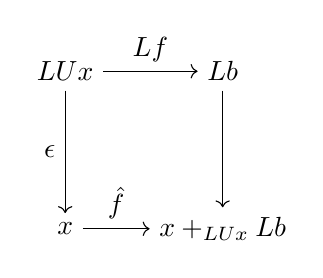
\begin{tikzpicture}
      \node (ul) at (0,2) {$ \L \U x $};
      \node (ll) at (0,0) {$ x $};
      \node (ur) at (2,2) {$ \L b $};
      \node (lr) at (2,0) {$ x +_{\L\U x} \L b$};
      \draw [->] (ul) to node [left] {$ \epsilon $} (ll);
      \draw [->] (ul) to node [above] {$ \L f $} (ur);
      \draw [->] (ll) to node [above] {$ \hat{f} $} (lr);
      \draw [->] (ur) to (lr);
    \end{tikzpicture}
  \]
  is the cocartesian lift. There is a string of
  isomorphisms
  \[
    \U ( x +_{\L\U x} \L b ) \cong
    \U x +_{\U\L\U x} \L b \cong
    \U x +_{\U x} b \cong
    b
  \]
  whose composite we call $ h $.  Then
  \[
    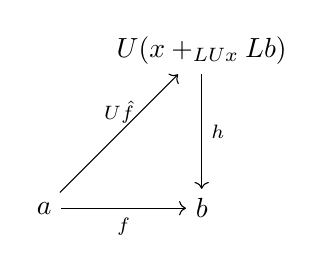
\begin{tikzpicture}
      \node (a) at (0,0) {$ a $};
      \node (b) at (2,0) {$ b $};
      \node (c) at (2,2) {$ \U ( x+_{\L\U x} \L b ) $};
      \path[->,font=\scriptsize]
      (a) edge node[below]{$ f $} (b)
      (a) edge node[above]{$ \U\hat{f} $} (c)
      (c) edge node[right]{$ h $} (b);
    \end{tikzpicture}
  \]
  commutes, and so $ \hat{f} $ is an appropriate
  lift. It remains to show that $ \hat{f} $ is
  cocartesian.

  Consider a $ \X $-arrow $ g \from x \to y $
  with a $ \A $-arrow
  $ \theta \from \U( x +_{\L\U x} \L b ) \to \U y $ so
  that $ \theta \U \hat{f} = \U g $.  Can we
  uniquely lift $ \theta $? Set up the diagram
  \[
    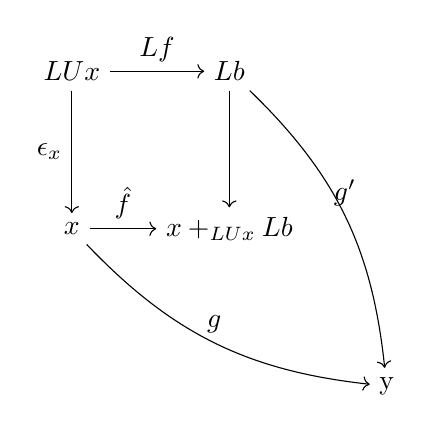
\begin{tikzpicture}
      \node (ul) at (0,2) {$ \L\U x $};
      \node (ll) at (0,0) {$ x $};
      \node (ur) at (2,2) {$ \L b $};
      \node (lr) at (2,0) {$ x +_{\L\U x} \L b$};
      \node (comp) at (4,-2) {y};
      \draw [->] (ul) to node [left] {$ \epsilon_x $} (ll);
      \draw [->] (ul) to node [above] {$ \L f $} (ur);
      \draw [->] (ll) to node [above] {$ \hat{f} $} (lr);
      \draw [->] (ur) to (lr);
      \draw [->] (ll) to [bend right=20] node [above] {$ g $} (comp);
      \draw [->] (ur) to [bend left=20] node [above] {$ g' $} (comp);
    \end{tikzpicture}
  \] 
  where $ g' \bydef \epsilon_y \L\theta \L h^{-1} $.
  To show the outer square commutes, it suffices
  to show that $ g' \L f $ and $ g \epsilon_x $
  have the same image under the adjunction homset
  correspondence.  We have
  \[
    g' \circ \L f =
    \epsilon_y \circ \L\theta \circ \L h \circ \L f
    \mapsto
    \U\epsilon_y \circ \U\L\theta \circ \U\L h
      \circ \U\L f \circ\eta_{ux}
    = \theta \circ h \circ f   
    = \theta \circ \U \circ \hat{f} 
    = \U g
  \]
  and 
  \[
    g \epsilon_x
    \mapsto
    \U g \circ \eta_{\U x}
    = \U g
  \]
\end{proof}

We now intersect the hypothesis of Propositions
\cref{thm:street-opfib-to-corefl} and
\cref{thm:corefl-to-street-opfib} to provide the
main result of this section.

\begin{thm}
  \label{thm:main-theorem-street-version}
  Suppose that $ \A $ and $ \X $ have chosen
  initial objects and pushouts. Then $ \U $ is a
  coreflector if and only if $ \U $ is a Street
  opfibration.  
\end{thm}

\begin{comment}
\section{Miscellaneous Theorems}

% \begin{thm}[Freyd's general adjoint functor theorem]
% \label{thm:GAFT}
% 	A functor $ F \from X \to Y $ is a right adjoint if  $ x $ is complete, locally small, and $ F $ satisfies the \emph{solution set condition}. The latter says, for any $ Y $-object $ y $, there exists a small set $ I $ indexing a collection of $ X $-objects $ {x_i}_I $ and $ Y $-arrows $ {f_i \from y \to F ( x_i ) } $ such that every $ F $-valued $ Y $-arrow $ y \to R x $ factors as $ Fg . f_k $ for $ k \in I $ and $ g \from x_k \to x $.
% \end{thm}

% \begin{proof}
% 	The proof is V.6.2 in CWM.  Define the left adjoint $ G \from Y \to X $ by $ G (y) \coloneqq x $ where $ y \to F x $ is initial in the comma category $ y \downarrow F $.  
% \end{proof}

% \begin{thm}[Gabriel-Zisman]
% \label{thm:GabZis}
% 	An adjunction $ \L \dashv R \from \cat{C} \leftrightarrow \cat{D} $. TFAE:
% 	\begin{enumerate}
% 		\item $ \L $ is full and faithful;
% 		\item the unit is an isomorphism;
% 		\item the induced comonad on $ \cat{D} $ is idempotent, $ \L $ is conservative, and $ R $ is essentially surjective.
% 	\end{enumerate}
% \end{thm}

{\daniel The following theorems were attempts at
  getting at an inverse of the RALI gives a
  St. opfibration.  But now with Theorem
  \ref{thm:street-opfib-to-corefl}, we probably
  don't need them.  Should we throw them away or
  keep them as nifty things?} {\chris Good question! If we are to keep, we should probably do so before our results and say how those would be reasonable things to start with, but instead we had to roam elsewhere for that and that reason!}

\begin{thm}
	Let $ \cat{D}$ be locally small and complete. Also let $ R \from \cat{D} \to \cat{C} $ be a continuous, surjective-on-objects Grothendiek opfibration.  Then $ R $ is a right adjoint.
\end{thm}

\begin{proof}
	We use \ref{thm:GAFT}.  Suffice to show the solution set condition holds.  Fix a $ C $-objects $ c $.  Then the indexing set is $ \ast $, the collection of $ D $-objects consists of a single object $ x_c $ over $ c $ (which exists by surjective-on-objects assumption), and the collection of $ \cat{C} $-arrows consists of the identity.  Any map $ f \from c \to Rd $ has a cocartesian lifting $ \hat{f} \from x_c \to x_{Rd} $ and $ f = R \hat{f} . 1_c $.
\end{proof}

\begin{thm}
	Let $ \cat{D}$ be locally small and complete. Also let $ R \from \cat{D} \to \cat{C} $ be a continuous, surjective-on-objects, conservative Street opfibration.  Then $ R $ is a right adjoint.
\end{thm}

\begin{proof}
	We use \ref{thm:GAFT}.  Suffice to show the solution set condition holds.  Fix a $ C $-objects $ c $.  Then the indexing set is $ \ast $, the collection of $ D $-objects consists of a single object $ x_c $ over $ c $ (which exists by surjective-on-objects assumption), and the collection of $ \cat{C} $-arrows consists of the identity.  For any map $ f \from c \to Rd $, there exists an essential cocartesian lifting $ \hat{f} \from x_c \to d' $ together with a $ \cat{C} $-isomorphism $ h \from Rd' \to Rd $ such that $ f = h . R \hat{f} $. But $ f = h . R \hat{f} = R \hat{h} . R \hat{f} . 1_c = R (\hat{h} . \hat{f}) . 1_c $ where $ h = R \hat{h} $ because $ R $ is conservative.
\end{proof}

\begin{thm}
	Let $ \cat{D}$ be locally small and complete. Also let $ R \from \cat{D} \to \cat{C} $ be a continuous, essentially surjective, conservative Street opfibration.  Then $ R $ is a right adjoint.
\end{thm}

\begin{proof}
	We use \ref{thm:GAFT}.  Suffice to show the solution set condition holds.  Fix a $ C $-object $ c $.  Then the indexing set is $ \ast $, the collection of $ D $-objects consists of a single object $ d' $ where $ \theta \from c \cong Rd' $ (which exists by essential surjectivity), and the collection of $ \cat{C} $-arrows is $ { \theta } $.  For any $ \cat{C} $-arrow $ f \from c \to Rd $, we have (by Street opfibrationness) $ f . \theta^{-1} \from Rd' \to c \to Rd $, a cocartesian essential lifting $ \hat{ f . \theta^{-1} } \from d' \to d'' $ in $ \cat{D} $, and an isomorphism $ h \from d \to d'' $ (by conservatism) such that $ f . \theta^{-1} = Rh . R \hat{ f . \theta^{-1} } $.  This implies, as required by GAFT, that $ f = R (h\hat{ f . \theta }) . \theta $.
\end{proof}

Thoughts about these assumptions. Here are the desired examples I can think of now: $ \cat{Set} $ together with $ \cat{Graph} $ or $ \cat{Top} $. The enriched over sets and completeness are both there. So is essential surjectivity. And reflection of isomorphisms.  The continuity is definitely needed, since it's necessary if $ R $ is a right adjoint. 

Go back to the right adjoint we had in the ``converse'' to the above theorem.  That is, we have a coreflection $ \L \dashv R \from \cat{C} \leftrightarrow \cat{D} $ where $ \L $ is left exact.  Of course this gives the continuity of $ R $. Essential surjectivity follows from Gabriel-Zisman. Is it a Street opfibration? $ \L $ is conservative, but is $ R $?

\begin{ex}
  No, $ R $ is not in general conservative.
  Consider the underlying node functor
  $ \Grph \to \Set $.  All $ \Grph $-endomorphisms
  on
  \[
    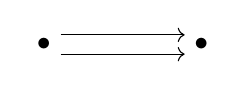
\begin{tikzpicture}
      \node (a) at (0,0) {$ \bullet $};
      \node (b) at (2,0) {$ \bullet $};
      \draw [->] (a.30) to (b.150);
      \draw [->] (a.-30) to (b.-150);
    \end{tikzpicture}
  \]
  are sent to the identity on $ 2 $.
\end{ex}
\end{comment}

\section{Categories of fibrations and adjunctions}

The key players here are subcategories of $\OpFib$ of those opfibrations that are fibred cocomplete, and of something like
$\Rali$ of ralis that strictly preserve all colimits.

{\chris Also, not sure if separate section for that, but we should try and include as many reasonable examples as possible. The quality rather
than the quantity is important I think! Grph Set the first such.}
{\chris Daniel mentioned we may want to do these things inside an arbitrary 2-category, at least for STreet fibration which is more natural and less evil? That would certainly be cool!}


\bibliographystyle{alpha}
\bibliography{references}



\end{document}

